\documentclass[a4paper,11pt]{scrartcl}
\usepackage[utf8]{inputenc}
\usepackage{float}
\usepackage{amsmath}
\newtheorem{theorem}{Theorem}
\usepackage{graphicx}
\usepackage{caption}
\usepackage{subfig}
\usepackage{pdfpages}
\usepackage{wrapfig}
\usepackage{subfig}

%opening
\subject{ Master's thesis\\
	Academic year 2022/2023 }
\title{Understanding the effect of opinions and behaviours on the spread of infectious diseases}
\subtitle{ }
\author{Riccardo Tessarin}
\date{ Email: riccardo.tessarin@studenti.unitn.it }



%% Stringhe per biblatex, compilare biber, pdflatex, biber pdflatex
\usepackage[english]{babel}
\usepackage[autostyle,italian=guillemets]{csquotes}                      
%% Per il corretto funzionamento di BibLatex
\usepackage[sorting=none,style=numeric-comp,backend=biber]{biblatex}
\addbibresource{bibliography.bib}

%pacchetto per i link cliccabili nel testo
\usepackage[hidelinks]{hyperref}
\hypersetup{ %impotazioni per i colori, in caso le volessi, a me non piacciono
	colorlinks=true,
	linkcolor=blue,
	filecolor=magenta,      
	urlcolor=cyan,
}

\urlstyle{same}


\begin{document}
	
	\maketitle
	\tableofcontents
	\pagebreak



\section{Introduction}
In human history the presence of disease, caused by parasite is always existed. 
Because of the lack of knowledge about medical science and the poor hygienical conditions the deaths caused by infections in history  have had dramatic repercussion on population life. During the bubonic plague of the 14th century for example 25 million of deaths were reported in Europe out of a population of 100 million. 
During the colonization of the Americas the disease imported by the Europeans is one of the main causes of the genocide of the local population. Diseases like smallpox and cholera were unknown in these countries and native americans have not antibodies to them. 



Not only diseases like these two have am incredible cost in term of human life. They have also effect on historical effect. Due to plague in fact in Europe starts the persecution against Jewish people, considered responsible of the illness spread. While in the Americas, the new infection were one of the element that permits at colonist to subdue the inhabitants. 
Others important epidemic, famous for their consequences were Spanish influenza, Smallpox, Typhus, HIV/AIDS and the more recent Covid-19. 
Because of these, is straightforward evidence of the effect that diseases have on our life.

Only in the last three centuries and just in the most developed countries, like Europe and North America, a significant increase in life expectancy have been observed. The mortality is decreased, but the modification in social patterns and the develop of large cities, have had some consequence. It was increased in the $18^{th}$ and $19^{th}$ centuries the frequency and magnitude of epidemics. 
For this reason diseases are an inevitable agents that is involved in our life. Their implications do not concern only our health status. When we are sick, there are modification in our relationship, work, social life. There is also an economic cost to be healed. Only in few nations worldwide treatment is covered free of charge by the state. In the majority, be ill can result in having to sustain excessive cost. Often due to this, people going into debit or to not take care. 
Nowadays, but also in the past when a new disease appears it is very important try to understand its origin, the biological mechanism under its spread, comprehend its resistance to existent drugs and so on. In practice collect all the information available to understand what is happening.  
These are part of the epidemiological investigation. Other key dimensions are for example genetic resistance, selective pressure of a disease on different human communities, the mechanism underline the acquisition of immunity. Using this knowledge epidemiology try to make a step further of only reconstruct the cause behind the development of a disease: model how can evolute during time. 
\begin{figure}[hbt!]
	\centering
	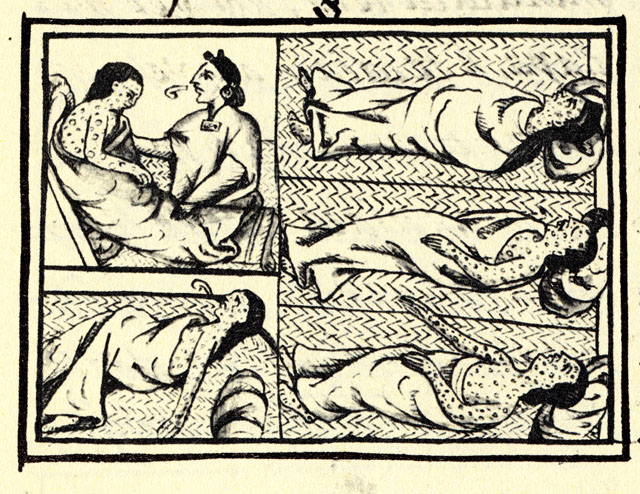
\includegraphics[width=0.4\linewidth]{images_introduction/FlorentineCodex_smallpox}
	\caption[smallpox on native Americans]{Representation of smallpox disease on the Mexican population in the $XIV$ century. Figure from \cite{Sahagun1965}. }
	\label{fig:florentinecodexsmallpox}
\end{figure}
There is a lot of interest about this topic both from a scientific perspective and also for public society regulations.
Develop a model that can give us the capability of estimate phenomena like the spread of a disease have a multitude of effects and outcomes on the society.  Social and economic costs are related to every illness, but develop instruments to better understand its impact can avoid the losses of human life and permit to have less serious effect on the society. 
A first simple example, that can help to understand the beneficial effect of study epidemics is the possibility to develop instruments that can permits to consider the specificity of each different disease with "simple" parameters and obtain information like:

\begin{itemize}
	\item is this disease so infective that can cause a pandemic?
	\item what are the threshold conditions that can cause and outbreak? 
\end{itemize}


At a first look the problem can seem simple. Unfortunately, the creation of a model capable of perform an evaluation like the one explained above, suitable for every disease is a problem for which there is not still a solution. 
Every research about the creation of a model that try to represent a real phenomenon must confront with the necessity to simplify, while trying to not loss in accuracy. 
So, in a century of research, many different aspects regarding an epidemic have been considered. The scientist try to catch the most significant ones to develop their model and then figure out if it is capable to give them insights about the considered disease. 
% Qui sarebbe carino iniziare con un discorso che spieghi un po' gli obbiettivi del lavoro 

 

% ! Ci sta inizialmente concentrarsi sulle epidemie, ma  devi intrudurre anche il secondo macro filone, quello delle opinioni. é uno spin off metodologico del primo, quindi gli stumenti matematici poi sono simili, ma va detta anche questa cosa. E poi sulle opinioni hai visto quante sfumature diverse esistono sul come considerarle e anche questo è da tenere in considerazione. 


\subsection{ Epidemiologic research historical background}
% Se ti piace l'idea di fare un piccolo excursus storico, va bene. Le info principali sono:
% 1- primo lavoro di Bernoulli
% 2- lavori di Hamer (1906) mass action principle, epidemic description in discrete time 
% 3- Ross, formulation in continous time 
% 4- Kermack and Mc Kendrick (1927) che danno risultato bello perchè introducono "legge" del thresold di una epidemia
% Dopo aver scritto quest'ultimo evento hai il LA per parlare di come funziona un mean field model. 

The research field regarding the development of technique to understand how epidemics can evolve during time has a history starting back in the 20th century. The first important discovery in this field must be attributed to the scientists that find the mechanism used by disease to spread. 
A first innovative work is the one done by John Snow, that during an epidemic of Cholera in London in 1854 successfully determined the source of the infection, even without knowing its etiological agent. Then advancing in the microbiological research is conducted by Pasteur and Koch. They found the etiological agent of disease, enabling the possibility to treat and prevent people from an infection. 
Then, Hamer work in 1906 added a first major theoretical contribution. He formulated a theory about the correlation between the course of an epidemic and the interaction, contact ratio, between susceptible and infectious individuals. It is the so called “mass -action” principle. The number of contacts between these two groups determines the spread rate of the disease. 
This law originally written in discrete time, is then updated in 1908 by Ross, that re-written it  in continuous time. For the first time the problem can be studied using a clearly, well defined mathematical theory. Then the contributions of Kermack and McKendrick in 1927 add another fundamental principle to the modern epidemiology. They formulated a threshold theory explaining which condition can generate the development of an epidemic. The theorem affirms that a certain value must be exceed, depending on the proportion of susceptible and infectious individual. Controlling this value permits to understand if the number of infections will increase, until a peak is reached or if the epidemic is a descendent phase \cite{Mata2021}, \cite{Anderson_82}. 
Their contribution with the mass action principle represents the base for the mean field model theory, that will be presented and analysed in section REF. 



 

\subsection{Epidemiological theory foundations}

Definition of the theoretical basis and main concepts that will be used in the present work. 

\subsubsection{Micro and Macro parasite}


%Since the milestone work of Kermack and Mc Kendrik a century is almost passed.

\newpage
\printbibliography[heading=bibintoc]

\end{document}